% !TeX program = pdflatex
% ============================================================================
% HACE: Addressing Viability Failure in Sequential Reinforcement Learning
%       with Homeostatic Auxiliary Rewards
%
% CSCI 2951X Course Project — Spring 2026, Brown University
%
% To compile:
%   pdflatex main_zh.tex && pdflatex main_zh.tex
% ============================================================================

\documentclass[sigplan,10pt]{acmart}

% 仅增加 pdfLaTeX 中文支持；不改变 acmart 的标题、章节或双栏样式。
\usepackage{CJKutf8}

\settopmatter{printfolios=false,printacmref=false}
\setcopyright{none}
\acmConference[CSCI 2951X]{CSCI 2951X 课程项目}{2026 年春季}{美国罗得岛州普罗维登斯}
\acmYear{2026}
\acmDOI{}
\acmISBN{}
\acmPrice{}

% ── Packages ─────────────────────────────────────────────────
\usepackage{booktabs}
\usepackage{enumitem}
\usepackage{amsmath,amssymb}
\usepackage{multirow}
\usepackage{subcaption}
\usepackage{xcolor}
\usepackage{hyperref}
\usepackage{makecell}
\usepackage{array}


% ── Notation ─────────────────────────────────────────────────
\newcommand{\setpoint}{H^*}
\newcommand{\energy}{E}
\newcommand{\drive}{d}
\newcommand{\reward}{r}
\newcommand{\hace}{\textsc{Hace}}
% 共用图表尚未同步到当前项目时显示占位框，而不中断整篇论文的编译。
% 图文件补齐后会自动恢复为与英文稿完全相同的插图。
\newcommand{\sharedfigure}[2][]{%
  \IfFileExists{#2}{\includegraphics[#1]{#2}}{%
    \fbox{\parbox[c][3.2cm][c]{0.92\linewidth}{\centering
      缺少共用图表：\texttt{\detokenize{#2}}}}}}

% ============================================================================
\begin{document}
\begin{CJK*}{UTF8}{gbsn}

\title{HACE：以稳态辅助奖励应对序列强化学习中的生存可行性失效}

\newcommand{\browncsaffiliation}{%
  \affiliation{%
    \department{计算机科学系}
    \institution{布朗大学}
    \city{普罗维登斯}
    \state{罗得岛州}
    \country{美国}}}

\author{Ziyu Kong}
\browncsaffiliation
\email{ziyu\_kong@brown.edu}

\author{Shihang Gui}
\browncsaffiliation
\email{shihang\_gui@brown.edu}

\author{Ruth Ukubay}
\browncsaffiliation
\email{ruth\_ukubay@brown.edu}

\author{Meiyi Song}
\browncsaffiliation
\email{meiyi\_song1@brown.edu}

% ============================================================================
\begin{abstract}
% ============================================================================

持续强化学习（continual reinforcement learning，CRL）研究长期以来几乎完全聚焦于
\emph{灾难性遗忘}，即神经网络在适应新任务时丧失既有技能的现象。在智能体必须管理共享
生理资源的具身环境中，本文识别出一种与之互补的失效模式：\emph{生存可行性失效}。
发生该失效时，智能体会耗尽内部资源，并在具备学习新任务的机会之前死亡。弹性权重巩固
（Elastic Weight Consolidation，EWC）、经验回放（Experience Replay，ER）等现有
持续强化学习技术着眼于参数保持或数据复用，而非资源状态管理，因此无法直接应对生存可行性
失效。为此，本文提出 \hace{}（Homeostatic Auxiliary for Continual Environments，
面向持续环境的稳态辅助机制）：一种基于稳态驱力降低的任务不变辅助奖励。该方法无需针对
具体任务进行专门设计，便可促使智能体主动管理能量。我们在包含 9 种智能体变体的 10 任务
资源继承基准上开展实验，并以 5 任务的“资源重置--资源继承”析因研究作为补充。结果表明，
\hace{} 智能体的任务边界可解性约为非稳态基线的 3 倍，且在任务切换时保留的能量约为后者的
3--5 倍；相比之下，传统持续强化学习方法在本文的生存可行性指标上并未优于无保护基线。
进一步地，将 \hace{} 与 EWC 结合能够同时改善生存可行性与知识保持。这一结果表明，在具身
持续强化学习中，维持生存与缓解遗忘是两个部分可分离的问题维度。

\end{abstract}

\maketitle

% ============================================================================
\section{引言}
\label{sec:intro}
% ============================================================================

部署于持续学习场景中的强化学习智能体，必须在适应不断变化的目标时保留已经习得的能力。
当前持续强化学习研究通常将这一挑战近乎完全归结为\emph{灾难性遗忘}，即模型在新任务训练
过程中发生参数覆盖，从而丧失旧知识~\cite{Parisi2019,kirkpatrick2017,continualworld2021}。
围绕这一问题，研究者已经提出了丰富的方法，包括弹性权重巩固
（EWC~\cite{kirkpatrick2017}）、经验回放（ER~\cite{rolnick2019}）以及渐进式网络
架构~\cite{rusu2016} 等。这些方法的评估重点，通常是智能体在学习新任务后能否维持旧任务
上的性能。

本文认为，对遗忘问题的集中关注掩盖了具身序列学习场景中另一种同样关键的失效模式：
\textbf{生存可行性失效}。当环境施加跨任务共享的生理约束时——例如智能体每执行一步动作，
其内部能量都会下降——任务切换本身便可能带来致命后果。若智能体在完成任务 $T_i$ 时仅剩
极少能量，那么进入任务 $T_{i+1}$ 后，它可能没有足够资源存活到能够有效探索和学习的阶段。
对于一个在新任务开始后的前三步内便死亡的智能体，无论施加多强的权重正则化，或回放多少
历史转移数据，都无法弥补其生存条件的缺失。

以本文基准中的具体任务切换为例：智能体首先在 \textsc{Conservation} 任务中训练。该任务
具有较高的单步能耗，要求智能体采取高效策略；随后，智能体切换至 \textsc{Sprint} 任务，
后者的时间限制极短，要求快速完成目标。在资源继承边界条件下，任务切换时能量不会被重置。
因此，智能体可能以严重不足的能量进入 \textsc{Sprint}，且没有可供探索的时间，最终立即
死亡。尽管 EWC 可以完整保留 \textsc{Conservation} 阶段的重要权重，但如果智能体无法
存活，这些权重便无法发挥作用。

本文的贡献主要包括三个方面。第一，我们形式化提出具身持续强化学习中的
\textbf{生存可行性失效}，将其界定为区别于灾难性遗忘的独立失效模式，并说明传统持续强化
学习方法并未直接作用于这一问题（第~\ref{sec:method} 节）。第二，我们提出 \textbf{\hace{}}
方法：一种基于稳态驱力降低的任务不变辅助奖励。该奖励无需逐任务设计，即可在所有任务中
激励智能体进行能量管理。第三，我们构建了一个包含 9 种智能体变体和人工编排任务序列的
\textbf{10 任务序列网格世界基准}，从而能够系统研究上述两类失效模式
（第~\ref{sec:setup} 节）。实验结果（第~\ref{sec:results} 节）表明，\hace{} 能够帮助
智能体在任务切换过程中维持生存可行性，而传统持续强化学习方法在本文基准中未能改善相应的
生存指标。


% ============================================================================
\section{相关工作}
\label{sec:related}
% ============================================================================

\paragraph{持续强化学习。}
EWC~\cite{kirkpatrick2017} 通过基于 Fisher 信息加权的惩罚项约束重要参数；
ER~\cite{rolnick2019} 在新任务训练过程中穿插回放旧任务的转移数据；渐进式网络
~\cite{rusu2016} 则冻结已有网络列，并为每项新任务增加模型容量。这些方法已在
Continual World~\cite{continualworld2021}、CORA~\cite{cora2022} 等基准上得到广泛评估。
然而，在此类基准中，单回合终止通常不受资源约束影响。本文指出，这种评估范式并未直接检验
生存可行性失效。

\paragraph{稳态强化学习。}
Keramati 与 Gutkin~\cite{keramati2014} 将奖励形式化为智能体内部状态相对于稳态设定点的
偏差缩减，并由此产生风险规避与预期性调节行为。Yoshida~\cite{yoshida2018,Yoshida} 将
这一框架扩展至深度强化学习，并进一步将其与元强化学习联系起来。Konidaris 与
Barto~\cite{konidaris2006} 则提出了自适应动机系统。然而，既有研究大多聚焦于单一环境或
缓慢变化的环境，尚未检验稳态目标能否改善序列任务学习。

\paragraph{迁移学习与辅助奖励。}
后继特征方法~\cite{Barreto} 将价值函数分解为可复用的环境动力学表征与任务特定权重。
Tomov 等人~\cite{Tomov} 发现，人类能够跨任务复用既有策略，并提出任务描述可以植根于
生理状态；\hace{} 将这一观点落实为可操作的方法。与好奇心驱动奖励~\cite{pathak2017}
或像素控制~\cite{jaderberg2017} 不同，\hace{} 的直接目标并非促进探索或表征学习，而是
\emph{维持生存可行性}。


% ============================================================================
\section{生存可行性失效与 HACE}
\label{sec:method}
% ============================================================================

\subsection{序列任务设定}

本文考虑智能体依次学习任务序列 $T_1, \ldots, T_n$ 的情形。所有任务共享同一动作空间，
并共享内部能量变量 $\energy_t \in [0, \energy_{\max}]$。智能体每执行一步动作需消耗
$c_{\text{step}}$ 单位能量；当 $\energy_t \leq 0$ 时，回合因智能体死亡而终止。各任务在
网格布局、危险区域、食物来源、墙体结构和能量收支等方面有所不同
（见第~\ref{sec:setup} 节）。在任务边界处，智能体保留其网络参数。能量状态则由
\emph{边界模式}决定：\textbf{重置}模式将能量重新初始化为新任务的默认值；
\textbf{继承}模式保留上一任务结束时的能量。后者更符合生态情境，也最容易暴露生存可行性
失效。

\subsection{生存可行性失效}

若智能体完成任务 $T_i$ 后的期望终止能量，不足以支持其在 $T_{i+1}$ 中进行有效探索，
则称智能体在任务边界 $T_i \to T_{i+1}$ 处发生生存可行性失效：
\begin{equation}
  \mathbb{E}_{\pi_i}\!\left[\energy_{T_i}^{\text{terminal}}\right]
  \;\!<\;\! \energy_{\text{viable}}^{(i+1)}.
\end{equation}
在这种情况下，智能体会在新任务开始后的最初几步内死亡，所观察到的轨迹大多短暂且以死亡
告终，因而难以获得与成功行为有关的有效学习信号。该现象与灾难性遗忘存在根本差异：遗忘是
一个\emph{参数层面}的问题，即旧权重被新任务训练覆盖；生存可行性失效则是一个
\emph{轨迹层面}的问题，即智能体的存活时间不足以支撑学习。EWC 即便能够完好保护旧权重，
也无法迫使智能体节约能量。ER 虽然会回放旧转移，但这些转移未必能够改善智能体在新任务
边界处已经耗竭的资源状态。L2 正则化仅约束参数幅值，同样不提供任何生存信号。因此，这些
方法所针对的是参数或数据的保持，而生存可行性失效取决于智能体抵达任务边界时实际形成的
资源状态。

在实验中，我们通过任务边界可解性对上述阈值进行经验化刻画：具体而言，考察当前策略从
上一任务的终止能量分布出发时，能否完成下一任务。

\subsection{稳态驱力降低}

遵循 Keramati 与 Gutkin~\cite{keramati2014} 的定义，我们将内部驱力表示为当前能量与
稳态设定点 $\setpoint$ 之间的距离，即 $\drive_t = |\setpoint - \energy_t|$。
\hace{} 的辅助奖励定义为单步驱力降低量：
\begin{equation}
  \reward_t^H \;=\; |\setpoint - \energy_t| \;-\; |\setpoint - \energy_{t+1}|.
  \label{eq:drive}
\end{equation}
当某一动作使智能体更接近稳态时，该信号为正，例如能量不足时获取食物；当动作增大智能体
与稳态的偏差时，该信号为负。其函数形式具有\emph{任务不变性}：在不同任务中，智能体始终
接收相同的驱力降低信号，而能量依据各任务的能量上限进行归一化。该信号同时具有
\emph{稠密性}，能够逐步提供反馈；其设计也具有\emph{生物学依据}，与生物体的驱力降低机制
相对应~\cite{keramati2014,konidaris2006}。

完整的 \hace{} 奖励将该辅助项与任务特定奖励结合：
$\reward_t^{\text{HACE}} = \alpha \cdot \reward_t^{\text{task}} + \reward_t^H$。
默认情况下，$\alpha = 1.0$ 且 $\setpoint = \energy_{\text{cap}}$。在本文基准中，将稳态点
设为能量上限，使 \hace{} 成为一种保守的能量维持信号：智能体因避免以资源耗竭状态抵达
任务边界而获得奖励，而非仅追求任务奖励最大化。本文采用这一具体设定，是因为环境中的核心
风险来自能量耗竭引发的死亡；在其他领域中，则可能需要采用中间稳态点或可自适应的稳态点。
由于 \hace{} 作用于\emph{奖励层面}，而 EWC/ER 分别作用于\emph{权重层面}和
\emph{数据层面}，二者天然具有互补性。因此，智能体 I（\hace{}+EWC）将两类方法结合，
以同时应对生存可行性失效与灾难性遗忘。


% ============================================================================
\section{实验设置}
\label{sec:setup}
% ============================================================================

\subsection{任务基准}

我们设计了 12 个结构各异的网格世界任务。所有任务共享相同的能量动力学，但在空间布局、
危险区域、食物位置、墙体、门控机制、单步能耗和能量容量等方面存在差异。
表~\ref{tab:tasks} 汇总了完整的任务集合。每个任务均实现为 Gymnasium 环境：
智能体在离散网格中移动，每执行一步动作均消耗能量；通过收集食物恢复能量，并在规避
危险单元的同时穿越墙体和门控结构。回合在智能体成功抵达出口或能量耗尽时终止。

\begin{table}[t]
\centering
\caption{任务集合。所有任务共享 4 种移动动作，并在智能体死亡时终止。
$c_s$ 表示单步能耗，F 表示食物数量，H 表示危险区域数量。}
\label{tab:tasks}
\small
\setlength{\tabcolsep}{3.8pt}
\begin{tabular}{@{}lcccccl@{}}
\toprule
\textbf{任务} & \textbf{网格} & $\energy_0$ & $c_s$ &
\textbf{F} & \textbf{H} & \textbf{核心挑战} \\
\midrule
Reach          & 5 & 15 & 1 & 1 & 0 & 路径导航 \\
Recharge       & 5 &  8 & 1 & 1 & 0 & 必须进食以维持生存 \\
Hazard Cross   & 5 & 12 & 1 & 1 & 2 & 危险规避 \\
Detour         & 5 &  9 & 1 & 1 & 2 & 进食与规避 \\
Wall Maze      & 6 & 14 & 1 & 1 & 0 & 空间规划 \\
Dual Food      & 6 & 10 & 1 & 2 & 1 & 稀缺条件下的决策 \\
Haz.~Gauntlet  & 6 & 14 & 1 & 1 & 4 & 密集危险区域 \\
Conservation   & 5 & 20 & 2 & 1 & 1 & 高单步能耗 \\
Endurance      & 7 & 16 & 1 & 1 & 2 & 长距离路径 \\
Collect Exit   & 6 & 14 & 1 & 1 & 2 & 门控机制 \\
Sprint         & 5 & 14 & 1 & 1 & 0 & 极短时间限制 \\
Gaunt.~Refuel  & 7 & 16 & 1 & 2 & 4 & 综合运用全部技能 \\
\bottomrule
\end{tabular}
\end{table}

我们人工编排了三种 10 任务顺序：\textbf{$\alpha$（能量迁移）}序列使能量管理技能
逐步累积；\textbf{$\beta$（安全迁移）}序列优先学习危险规避技能；
\textbf{$\gamma$（干扰）}序列则有意安排策略相互冲突的任务切换，例如
Conservation $\to$ Sprint。完整任务顺序见附录~\ref{app:sequences}。

\subsection{智能体配置}

我们设计了 9 种智能体变体（表~\ref{tab:agents}），系统改变奖励信号、能量观测、
持续强化学习方法和训练模式。\textbf{任务预言机（Task Oracle）}作为性能参照：
它不采用序列任务设定，而是分别在每个任务上独立训练，本文希望 \hace{} 的成功率尽可能
接近这一参照。\textbf{仅任务奖励（Task-only）}是基础智能体，只接收任务特定奖励。
\textbf{能量感知（Energy-aware）}智能体额外观测能量，但策略更新仍仅使用任务奖励。
智能体 C 与 D 均采用单步驱力降低形式的稳态奖励，其中 \textbf{\hace{}} 同时结合任务奖励
和稳态奖励，而\textbf{纯稳态（Pure Homeostatic）}智能体完全舍弃任务奖励。
智能体 F、G 和 H 分别采用旨在缓解灾难性遗忘的持续学习方法。最后，
\textbf{\hace{}+EWC} 同时处理生存可行性与遗忘问题，用以检验两类机制的互补关系。
所有智能体均采用相同的 DQN 架构，包括含 128 个隐藏单元的两层多层感知机和
$\varepsilon$-贪心探索策略；详细设置见附录~\ref{app:hyperparams}
和附录~\ref{app:obs}。

\begin{table}[t]
\centering
\caption{智能体配置。TR：任务奖励；EO：能量观测；HR：稳态奖励；
CRL：持续强化学习方法；Seq：序列训练（参数继承）。}
\label{tab:agents}
\small
\setlength{\tabcolsep}{3.5pt}
\begin{tabular}{@{}llccccc@{}}
\toprule
\textbf{编号} & \textbf{智能体} & \textbf{TR} & \textbf{EO} &
\textbf{HR} & \textbf{CRL} & \textbf{Seq} \\
\midrule
A & Task-only          & \checkmark & --  & --  & --     & \checkmark \\
B & Energy-aware       & \checkmark & \checkmark & --  & --     & \checkmark \\
C & \textbf{HACE}      & \checkmark & \checkmark & \checkmark & --     & \checkmark \\
D & Pure Homeostatic   & --  & \checkmark & \checkmark & --     & \checkmark \\
E & Task Oracle        & \checkmark & \checkmark & --  & --     & -- \\
F & EWC                & \checkmark & \checkmark & --  & EWC    & \checkmark \\
G & L2                 & \checkmark & \checkmark & --  & L2     & \checkmark \\
H & Exp.~Replay        & \checkmark & \checkmark & --  & ER     & \checkmark \\
I & \textbf{HACE+EWC}  & \checkmark & \checkmark & \checkmark & EWC    & \checkmark \\
\bottomrule
\end{tabular}
\end{table}

\subsection{评价指标}

我们采用以下指标评价智能体：\textbf{当前任务成功率}，即评估回合中成功抵达出口的比例；
\textbf{阶段结束评估矩阵} $R_{i,j}$，表示完成任务 $T_i$ 的训练后在任务 $T_j$ 上的成功率；
\textbf{任务边界可解性}，即当前策略从任务 $T_i$ 的实际终止能量出发时能否完成
$T_{i+1}$；任务边界处的\textbf{平均终止能量}；以及标准的\textbf{遗忘量}
$F_j = \max_{i \geq j} R_{i,j} - R_{n,j}$。

\subsection{实验协议}

所有主要实验均在资源继承边界模式下采用 $\alpha$ 序列，这是最具挑战性的设置。
每个任务训练 600 个回合，每训练 50 个回合执行 40 个评估回合，每种智能体使用
10 个随机种子。结果以均值和标准差报告。第~\ref{sec:factorial} 节进一步比较
资源重置与资源继承两种边界条件。


% ============================================================================
\section{实验结果}
\label{sec:results}
% ============================================================================

\subsection{完整九智能体实验（10 任务 $\alpha$ 序列，资源继承）}
\label{sec:full_suite}

图~\ref{fig:learning} 给出了 9 种智能体在 10 任务序列上的学习曲线。为降低视觉干扰，
图中重点显示四种主要智能体：仅任务奖励（A）、\hace{}（C）、EWC（F）和
\hace{}+EWC（I），其余五种智能体以背景曲线呈现。

\begin{figure*}[t]
  \centering
  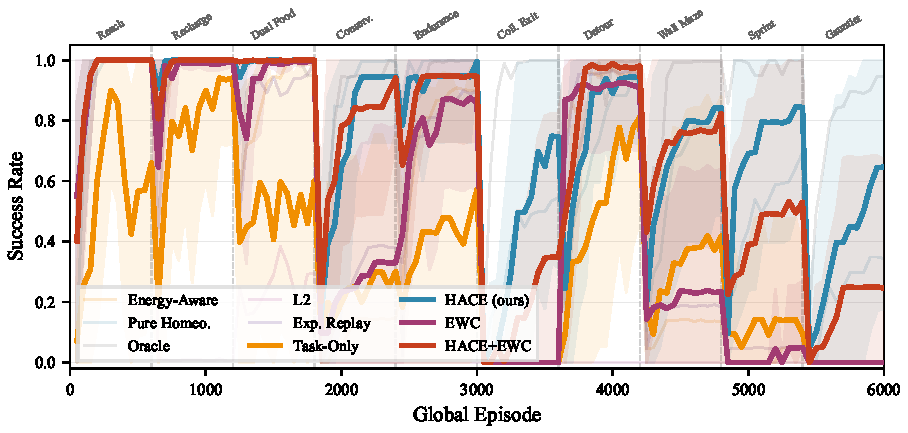
\includegraphics[width=\textwidth]{figures/fig_learning_curves.pdf}
  \caption{10 任务 $\alpha$ 序列在资源继承条件下的当前任务成功率。虚线表示任务边界。
  \hace{}（蓝绿色）和 \hace{}+EWC（朱红色）在任务切换后能够持续恢复，而仅任务奖励
  （琥珀色）和 EWC（淡紫色）在后期任务上出现性能崩溃。背景曲线表示其余智能体。
  曲线为 10 个随机种子的均值 $\pm\,1\sigma$。}
  \label{fig:learning}
\end{figure*}

学习曲线揭示了三个关键现象。第一，在序列后半段，传统持续强化学习方法 EWC、L2 和 ER
相较于无保护的仅任务奖励基线并未表现出生存可行性优势。在第 7--10 个任务
（从 Detour 到 Gauntlet Refuel）上，不使用稳态奖励的智能体成功率几乎降至零。
第二，\hace{} 智能体（C 和 I）能够在任务边界处的初始性能下降之后稳定恢复，表明稳态
奖励提供了持续的生存信号，使智能体能够在新任务中进行有效探索。第三，\hace{}+EWC（I）
在完整序列上表现最稳定，兼具 \hace{} 的生存可行性优势和 EWC 对早期任务权重的保护作用。

图~\ref{fig:boundary} 直接量化了上述生存机制。子图（a）给出了平均任务边界可解性：
\hace{} 和 \hace{}+EWC 的边界可解性约为 EWC、ER 和仅任务奖励智能体的 3 倍。
这一结果确认了生存可行性失效才是关键瓶颈——仅保护权重的持续学习方法并不能提高智能体
在下一任务中的存活能力。子图（b）揭示了其直接原因：\hace{} 智能体在任务边界处保留的
能量约为其他智能体的 3--5 倍，具体为 11.2 和 9.1，而其余智能体仅为 2--4；
更高的剩余能量使后续探索得以持续。

\begin{figure}[t]
  \centering
  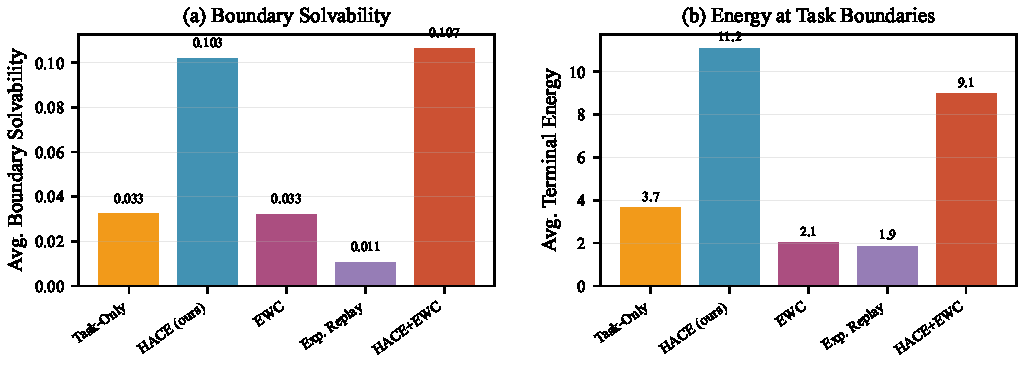
\includegraphics[width=\columnwidth]{figures/fig_boundary_energy.pdf}
  \caption{（a）9 次任务切换上的平均任务边界可解性；（b）任务边界处的平均终止能量。
  \hace{} 及其组合变体保留的能量约为所有持续学习基线的 3--5 倍，从而获得更高的
  任务边界可解性。}
  \label{fig:boundary}
\end{figure}

图~\ref{fig:heatmap} 展示了序列训练结束时的任务成功率矩阵。对比十分明显：
仅任务奖励智能体（A）在完成整个序列后，几乎无法保留任何任务上的性能；
\hace{}+EWC（I）在综合难度最高的 Gauntlet Refuel 上仍保持高于 0.25 的成功率，
并取得所有任务上最高的平均成功率 0.335。EWC（F）与 ER（H）虽然在一定程度上保护了
早期任务性能，例如在 Reach 上达到 0.40--0.53，但在最终任务上的成功率仍为零。
在非预言机智能体中，只有单独使用 \hace{} 的智能体（C）在 Gauntlet Refuel 上取得
显著成功，成功率超过 0.60。该任务要求综合运用导航、食物收集、危险规避和高效能量使用
四项能力。

\begin{figure}[!htb]
  \centering
  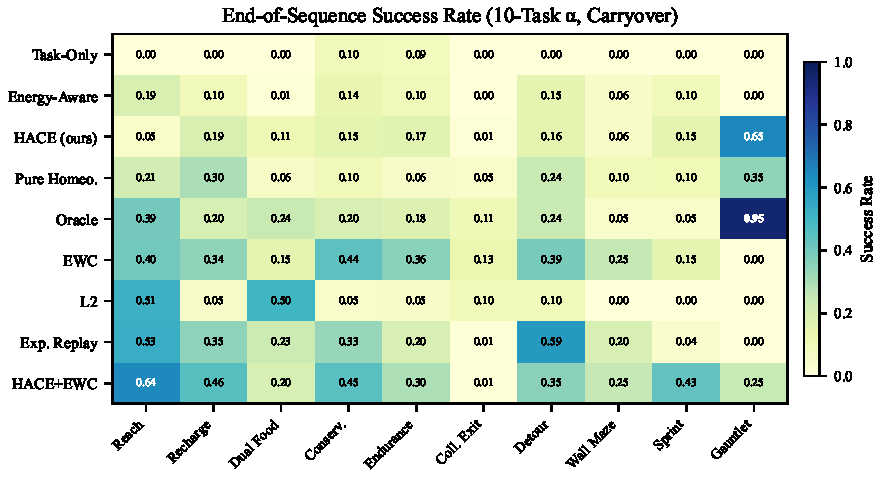
\includegraphics[width=\columnwidth]{figures/fig_performance_heatmap.pdf}
  \caption{资源继承条件下，10 任务 $\alpha$ 序列训练结束时的成功率矩阵
  （智能体 $\times$ 任务）。颜色越深表示成功率越高。\hace{}+EWC（最下行）取得最高的
  平均性能；\hace{}（C）是唯一能够完成 Gauntlet Refuel 的非预言机智能体。}
  \label{fig:heatmap}
\end{figure}


\subsection{资源重置与继承：分离生存可行性失效}
\label{sec:factorial}

为确认资源继承条件下的性能崩溃源于生存可行性失效，而非灾难性遗忘，我们在五任务先导
序列上开展了 $3 \times 2$ 析因实验，即 3 种奖励机制与 2 种边界模式的组合；
每个实验条件均使用 10 个随机种子。

\begin{figure}[!htb]
  \centering
  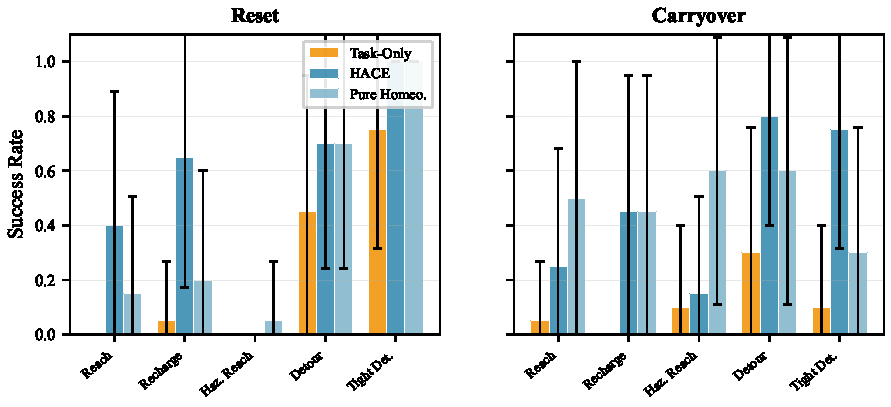
\includegraphics[width=\columnwidth]{figures/fig_viability_collapse.pdf}
  \caption{资源重置（左）与资源继承（右）条件下的最终评估结果。在重置条件下，各智能体
  表现相近；在继承条件下，仅任务奖励智能体（琥珀色）出现性能崩溃，而 \hace{}
  （蓝绿色）能够维持性能。相同权重在重置条件下仍可有效工作，说明性能崩溃源于
  生存可行性失效，而非遗忘。}
  \label{fig:collapse}
\end{figure}

图~\ref{fig:collapse} 提供了直接证据。在重置模式下，三种奖励机制的性能相近，
仅任务奖励智能体在 Detour 上达到 0.45--0.75 的成功率；在继承模式下，该智能体的
成功率降至 0.30，而 \hace{} 仍保持 0.80。关键在于，产生上述差异的是\emph{同一组网络
权重}，唯一变化是任务切换时是否重置能量。因此，灾难性遗忘不足以解释这一现象，
真正的瓶颈是生存可行性失效。稳态智能体在序列结束时维持了更高的终止能量
（2.95，而仅任务奖励智能体为 0.35），这直接提高了其在后续任务中的存活概率。


\subsection{MiniGrid 验证}
\label{sec:minigrid}

为检验 \hace{} 的优势能否推广至自定义网格世界之外，我们在并非为本研究专门设计的标准
MiniGrid 基准~\cite{minigrid} 中复现序列迁移实验。实验构建了一个难度逐步增加的五任务
序列：\textit{Reach}（在空房间中导航至目标）、\textit{Recharge}（必须收集食物才能
存活）、\textit{Hazard Reach}（熔岩阻断直接路径）、\textit{Detour}（同时要求食物收集
和危险规避）以及 \textit{Conservation}（单步能耗加倍，强调行动效率）。所有任务均采用
与自定义网格世界相同的能量动力学。我们在资源继承与资源重置两种边界模式下，对 5 种智能体
分别使用 10 个随机种子，每个任务训练 3000 个回合。

\paragraph{资源继承条件。}
图~\ref{fig:minigrid_carryover} 展示了学习曲线和阶段结束成功率。\hace{} 在前三个任务上
达到接近完美的成功率：Reach 为 100\%，Recharge 为 99.3\%，Hazard Reach 为 98.0\%；
在难度更高的任务上仍保持较高成功率，Detour 为 74.8\%，Conservation 为 71.0\%。
仅任务奖励智能体的性能则逐步下降，在 Conservation 上仅为 9.2\%。EWC、L2 和 ER
三种持续学习基线在第一个任务之后几乎完全崩溃，后续任务成功率接近零，尽管这些方法原本
专门用于防止遗忘。该结果进一步表明，权重正则化和经验回放作用于错误的抽象层级：
它们可以保持参数，却无法防止智能体以资源耗竭状态进入新任务。

\begin{figure*}[!ht]
  \centering
  \sharedfigure[width=\textwidth]{figures/fig_minigrid_carryover.png}
  \caption{MiniGrid 资源继承实验（10 个随机种子）。\emph{左：}五任务序列上的学习曲线。
  \hace{}（蓝色）是唯一能在 Conservation 任务上继续改善的智能体；仅任务奖励智能体
  （红色）在 Recharge 后显著退化，EWC、L2 和 ER 在首个任务后维持在接近零的水平。
  \emph{右：}阶段结束成功率。\hace{} 在五个任务上均保持较高成功率。}
  \label{fig:minigrid_carryover}
\end{figure*}


\paragraph{机制分析：资源继承与重置。}
图~\ref{fig:minigrid_mechanism} 比较了两种边界条件。在重置模式下，EWC、L2 和 ER
均显著恢复，并在五个任务上取得有竞争力的性能。“继承减重置”的差值图表明，资源继承会
损害所有智能体的性能，但持续学习基线受到的影响最大，在 Recharge 和 Hazard Reach 上
差值约为 $-1.0$；相比之下，\hace{} 在所有任务上的负向差值最小。这一结果直接确认，
\hace{} 的优势由能量通道所介导：移除资源继承，也就移除了暴露基线脆弱性的生存压力，
因此 \hace{} 的相对优势随之缩小。

\begin{figure*}[!ht]
  \centering
  \sharedfigure[width=\textwidth]{figures/fig_minigrid_mechanism.png}
  \caption{MiniGrid 机制分析（10 个随机种子）。\emph{左：}资源继承条件；
  \emph{中：}资源重置条件，持续学习基线性能恢复，证实问题在于生存可行性失效而非遗忘；
  \emph{右：}资源继承与重置的性能差值。\hace{} 的负向差值最小，表明其对边界条件
  具有更强稳健性。}
  \label{fig:minigrid_mechanism}
\end{figure*}

\section{扩展基准实验}
\label{sec:benchmark}

我们进一步在 Crafter、COOM 和 Continual World 三个序列强化学习基准上检验本文方法。
相较于各基准中的原始方法，\hace{} 智能体在这些环境中均表现出积极结果。

\subsection{Crafter}
\label{sec:crafter}

\begin{figure*}[htbp]
  \centering
  \sharedfigure[width=\textwidth]{figures/crafter_figure.png}
  \caption{\textbf{待补充：Crafter 实验的综合结果。}}
  \label{fig:crafter_figure}
\end{figure*}

\begin{figure}[htbp]
  \centering
  \sharedfigure[width=\columnwidth]{figures/crafter_learning_curves.pdf}
  \caption{\textbf{待补充：Crafter 实验的学习曲线。}}
  \label{fig:crafter_learning_curve}
\end{figure}

\subsection{COOM}
\label{sec:coom}

COOM 是一个三维环境持续强化学习基准，由目标各异的任务序列构成。我们在 CO8 任务序列上
评估原始 COOM PackNet 基线和本文的 \hace{}+PackNet 方法。该序列依次包含 Pitfall、
Arms Dealer、Hide and Seek、Floor is Lava、Chainsaw、Raise the Roof、Run and Gun
以及 Health Gathering。我们在 PackNet 基线上加入式~\ref{eq:drive} 定义的驱力降低奖励，
并将其与原任务奖励相加，从而实现 \hace{} 智能体。基线和 \hace{} 变体均使用 5 个随机
种子，每个任务训练 100 万个环境步。

如表~\ref{tab:hace_packnet_performance} 所示，\hace{} 辅助奖励使 Hide and Seek 与
Floor is Lava 的成功率分别提高 17\% 和 35\%。Pitfall 与 Raise the Roof 上也出现
轻微改善，增幅分别为 8\% 和 3\%，其余任务的成功率没有下降。这些结果与本文预期一致：
八个任务中，只有 Hide and Seek 与 Floor is Lava 允许智能体逐渐受到伤害，因此感知
健康状态的辅助奖励与其目标直接相关。Pitfall 与 Raise the Roof 虽然包含健康概念，
但主要失败机制是“立即死亡”，限制了驱力降低的作用。其余任务与健康状态几乎没有直接关联，
因而 \hace{} 对其性能影响较小。

\subsection{Continual World}
\label{sec:cw}


% ============================================================================
\section{讨论与结论}
\label{sec:discussion}
% ============================================================================

实验结果形成了三项对更广泛持续强化学习研究具有启示意义的发现。

\paragraph{生存可行性失效是一种独立且长期被忽视的失效模式。}
资源重置与继承对比实验（第~\ref{sec:factorial} 节）清楚表明，资源继承条件下的性能崩溃
并非灾难性遗忘，因为相同权重在资源重置条件下仍能成功完成任务。完整九智能体实验进一步
证实，EWC、L2 和 ER 等成熟持续学习方法在生存可行性指标上并不优于无保护基线。
这说明，通常假设能量无限且不存在死亡风险的标准持续强化学习评估范式，可能系统性忽略了
具身环境中最为紧迫的失效模式。

\paragraph{HACE 简洁有效，并与持续强化学习方法相互正交。}
\hace{} 辅助奖励（式~\ref{eq:drive}）只需对任意强化学习训练循环进行一行修改，
无需任务特定调参、额外参数或架构变更，却能将任务边界可解性提高约 3 倍，并使智能体 C
成为唯一能够完成 Gauntlet Refuel 的非预言机智能体，成功率达到 0.65。智能体 I
（\hace{}+EWC）兼具两类方法的优势：既获得 \hace{} 层面的生存可行性，又通过 EWC
保持早期任务知识，最终取得最高的总体平均成功率 0.335。这种互补性提示我们，可以对具身
持续强化学习问题作出原则性分解：\emph{维持生存}属于奖励层面，\emph{记住方法}属于权重
层面，二者是需要分别应对的独立维度。

\paragraph{局限性与未来工作。}
本文基准主要采用向量观测的网格世界；未来需要扩展至视觉输入和更丰富的三维环境，以检验
结论的普适性。所有主要结果均基于 DQN，使用策略梯度或 Transformer 架构进行复现能够
进一步增强证据。本文仅建模单一资源——能量，而现实智能体往往需要同时调节多个相互耦合的
驱力。此外，我们固定采用 $\setpoint = \energy_{\text{cap}}$，尚未研究按任务学习或动态
调整稳态设定点。尽管存在上述局限，本文的概念性贡献仍不依赖于具体环境复杂度：生存可行性
失效是传统持续学习方法无法直接解决的独立瓶颈；同时，\hace{} 的简洁性使其可以直接应用于
任何具有共享资源约束的具身序列强化学习场景。


% ============================================================================
\bibliographystyle{ACM-Reference-Format}
\begin{thebibliography}{99}

\bibitem{keramati2014}
Mehdi Keramati and Boris Gutkin.
Homeostatic reinforcement learning for integrating reward collection
  and physiological stability.
\emph{eLife}, 3:e04811, 2014.

\bibitem{yoshida2018}
Naoto Yoshida.
Homeostatic Agent for General Environment.
\emph{Journal of Artificial General Intelligence}, 8(1):1--22, 2018.

\bibitem{Yoshida}
Naoto Yoshida.
Meta-Reinforcement Learning in Homeostatic Regulation.
Extended abstract, Computational and Cognitive Neuroscience, 2025.

\bibitem{konidaris2006}
George Konidaris and Andrew Barto.
An Adaptive Robot Motivational System.
In \emph{Proc.\ 9th Intl.\ Conf.\ Simulation of Adaptive Behavior},
  pp.\ 346--356, 2006.

\bibitem{kirkpatrick2017}
James Kirkpatrick et~al.
Overcoming catastrophic forgetting in neural networks.
\emph{PNAS}, 114(13):3521--3526, 2017.

\bibitem{rolnick2019}
David Rolnick, Arun Ahuja, Jonathan Schwarz, Timothy Lillicrap, and
  Gregory Wayne.
Experience replay for continual learning.
In \emph{NeurIPS 32}, 2019.

\bibitem{rusu2016}
Andrei~A. Rusu et~al.
Progressive neural networks.
\emph{arXiv:1606.04671}, 2016.

\bibitem{Parisi2019}
German~I. Parisi, Ronald Kemker, Jose~L. Part, Christopher Kanan, and
  Stefan Wermter.
Continual lifelong learning with neural networks: A review.
\emph{Neural Networks}, 113:54--71, 2019.

\bibitem{continualworld2021}
Michal Wolczyk et~al.
Continual World: A robotic benchmark for continual RL.
In \emph{NeurIPS 34}, 2021.

\bibitem{cora2022}
Sam Powers et~al.
CORA: Benchmarks, baselines, and metrics as a platform for continual
  RL agents.
In \emph{CoLLAs}, 2022.

\bibitem{Barreto}
Andre Barreto et~al.
Successor features for transfer in RL.
In \emph{NeurIPS 30}, 2017.

\bibitem{Tomov}
Momchil~S. Tomov, Eric Schulz, and Samuel~J. Gershman.
Multi-task reinforcement learning in humans.
\emph{Nature Human Behaviour}, 5(6):764--773, 2021.

\bibitem{jaderberg2017}
Max Jaderberg et~al.
Reinforcement learning with unsupervised auxiliary tasks.
In \emph{ICLR}, 2017.

\bibitem{pathak2017}
Deepak Pathak et~al.
Curiosity-driven exploration by self-supervised prediction.
In \emph{ICML}, pp.\ 2778--2787, 2017.

\bibitem{minigrid}
Maxime Chevalier-Boisvert, Bolun Dai, Mark Towers, et~al.
Minigrid \& Miniworld: Modular \& Customizable Reinforcement Learning
  Environments for Goal-Oriented Tasks.
\emph{arXiv:2306.13831}, 2023.

\end{thebibliography}

% ============================================================================
% APPENDIX
% ============================================================================
\clearpage
\onecolumn
\appendix

\section{超参数}
\label{app:hyperparams}

表~\ref{tab:hyperparams} 列出了所有智能体共享的超参数，并同时给出 EWC 正则化系数
$\lambda$、ER 蓄水池容量等智能体特定参数。

\begin{table}[h]
\centering
\caption{训练超参数。}
\begin{tabular}{@{}ll@{}}
\toprule
\textbf{参数} & \textbf{取值} \\
\midrule
网络架构 & 两层 MLP，每层 128 个隐藏单元 \\
优化器 & Adam \\
学习率 & $5 \times 10^{-4}$ \\
折扣因子 $\gamma$ & 0.99 \\
批量大小 & 64 \\
回放缓冲区 & 20{,}000 条转移 \\
目标网络更新 & 每 25 个回合 \\
$\varepsilon$-贪心 & 300 个回合内从 1.0 降至 0.05 \\
每项任务的训练回合数 & 600 \\
评估频率 & 每训练 50 回合评估 40 回合 \\
\midrule
EWC $\lambda$（F、I） & 400.0 \\
EWC Fisher 样本数 & 1{,}000 \\
L2 $\lambda$（G） & 100.0 \\
ER 蓄水池（H） & 5{,}000 条转移，采样比例 0.5 \\
\hace{} 稳态设定点 & 各任务的 $\energy_{\text{cap}}$ \\
\hace{} 系数 & 1.0 \\
任务奖励系数 $\alpha$ & 1.0 \\
\bottomrule
\end{tabular}
\label{tab:hyperparams}
\end{table}


\section{任务序列定义}
\label{app:sequences}

表~\ref{tab:sequences} 列出了实验中人工编排的三种 10 任务顺序。序列 $\alpha$ 是正文
全部主要实验采用的任务顺序；序列 $\beta$ 和 $\gamma$ 预留用于未来的跨序列泛化分析。

\begin{table}[h]
\centering
\caption{三种完整的 10 任务顺序。}
\label{tab:sequences}
\begin{tabular}{@{}cp{0.88\textwidth}@{}}
\toprule
\textbf{序列} & \textbf{任务顺序} \\
\midrule
$\alpha$ & Reach $\to$ Recharge $\to$ Dual Food $\to$ Conservation $\to$
           Endurance $\to$ Collect Exit $\to$ Detour $\to$ Wall Maze $\to$
           Sprint $\to$ Gauntlet Refuel \\
\midrule
$\beta$  & Reach $\to$ Hazard Cross $\to$ Haz.~Gauntlet $\to$ Wall Maze $\to$
           Detour $\to$ Recharge $\to$ Sprint $\to$ Conservation $\to$
           Collect Exit $\to$ Gauntlet Refuel \\
\midrule
$\gamma$ & Conservation $\to$ Sprint $\to$ Haz.~Gauntlet $\to$ Reach $\to$
           Endurance $\to$ Dual Food $\to$ Hazard Cross $\to$ Collect Exit $\to$
           Recharge $\to$ Wall Maze \\
\bottomrule
\end{tabular}
\end{table}


\section{先导实验：五任务序列学习}
\label{app:pilot}

在开展完整的九智能体实验之前，我们首先实施了一项小规模先导实验，以验证核心假设。
实验训练两种智能体：一种是与智能体 A/B 相当的任务特定智能体，另一种是与智能体 D
相当的稳态智能体。二者依次学习五任务传统序列
Reach $\to$ Recharge $\to$ Hazard Cross $\to$ Detour $\to$ Sprint，
每项任务训练 600 个回合，并使用 10 个随机种子。

先导实验结果（图~\ref{fig:pilot}）显示出稳定的性能权衡。任务特定奖励能够更快学会早期
简单任务：在 Reach 上，任务特定智能体约 200 个回合即达到 0.6 的成功率，而稳态智能体
约需 400 个回合。另一方面，在更依赖资源管理和危险规避的后期任务中，稳态智能体能够达到
或超过任务特定智能体。训练结束后的保持性能显示，二者在 Hazard Cross 上的成功率分别为
0.90 和 0.70，在 Detour 上分别为 0.80 和 0.60。这一先导结果推动了正文所述的大规模
九智能体析因实验设计。

\begin{figure}[h]
  \centering
  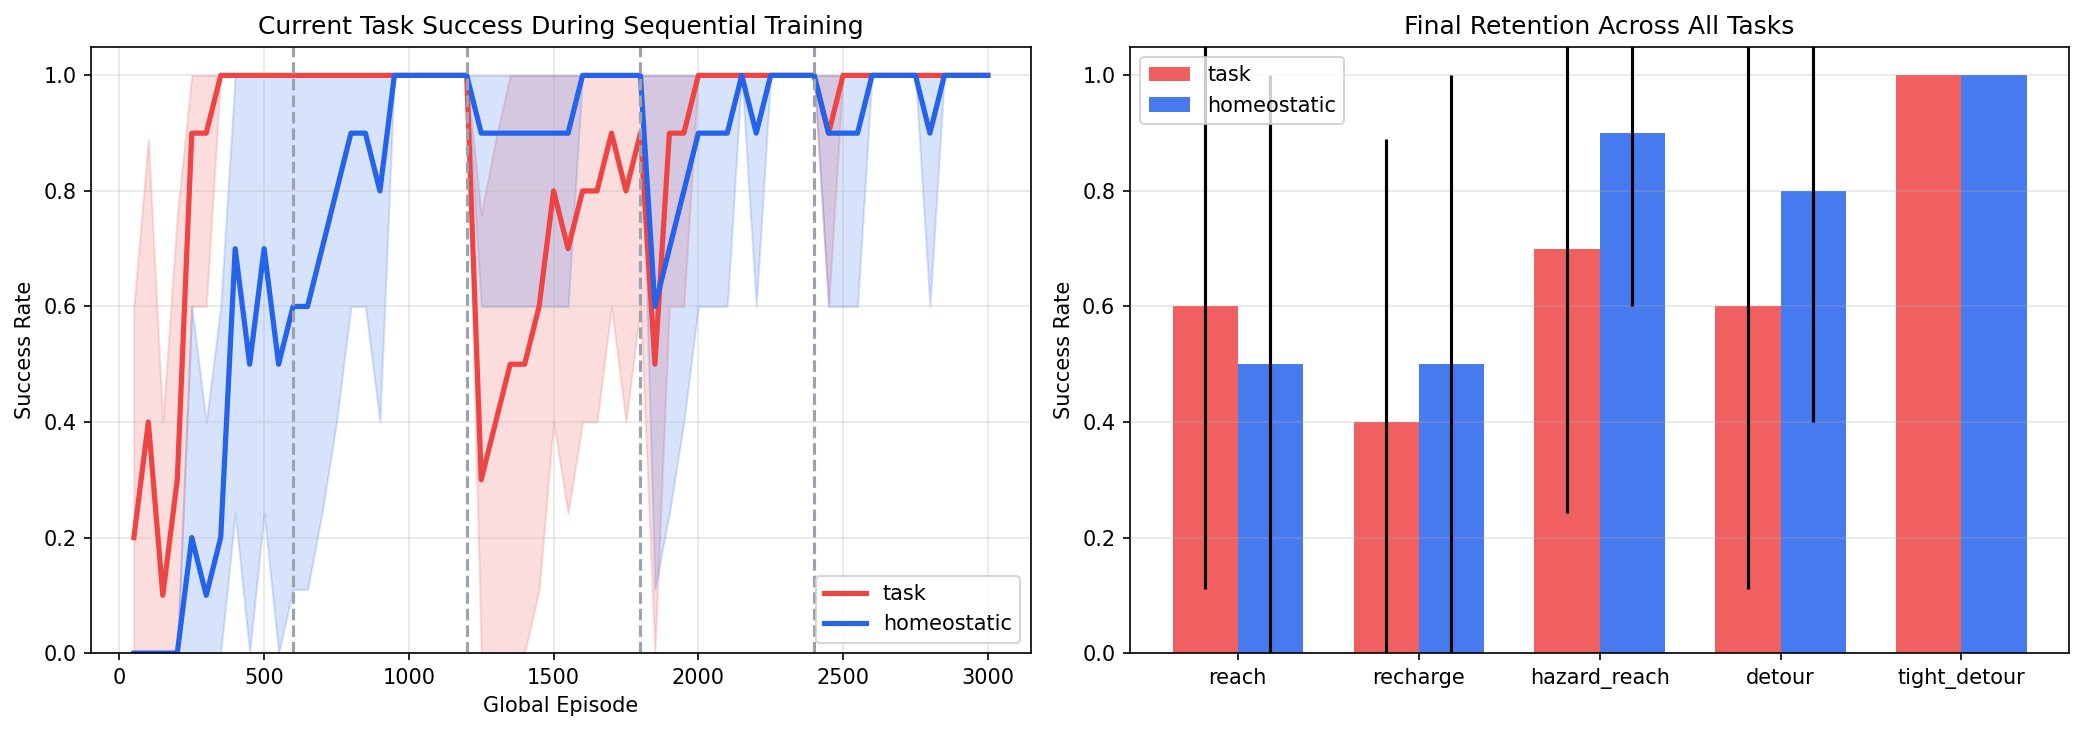
\includegraphics[width=0.85\textwidth]{figures/sequential_pilot.png}
  \caption{五任务序列先导实验。\emph{左：}序列训练期间的当前任务成功率。任务特定智能体
  （红色）学习早期任务更快；稳态智能体（蓝色）在后期任务上达到或超过其性能。
  \emph{右：}全部五项任务上的最终保持性能。稳态智能体在依赖资源的任务上表现出更强的
  保持能力（Hazard Cross：0.90 对 0.70；Detour：0.80 对 0.60）。}
  \label{fig:pilot}
\end{figure}


\section{观测空间细节}
\label{app:obs}

所有智能体均接收相同的 19 维向量观测（表~\ref{tab:obs}）。观测包含智能体位置、目标
位置、食物和危险区域的位置，以及尤为关键的智能体当前能量水平。所有空间特征均按网格尺寸
归一化，能量则按对应任务的能量上限归一化。

\begin{table}[h]
\centering
\caption{观测向量的组成。所有空间特征均归一化至 $[0,1]$。为区分奖励信号与观测内容
各自的作用，智能体 A 接收被掩蔽的能量值 $-1$。}
\label{tab:obs}
\small
\begin{tabular}{@{}cll@{}}
\toprule
\textbf{索引} & \textbf{内容} & \textbf{归一化方式} \\
\midrule
0--1 & 智能体位置（行、列） & $/$（grid\_size $-$ 1） \\
2--3 & 出口位置（行、列） & $/$（grid\_size $-$ 1） \\
4--6 & 食物 1：行、列、是否可用 & $/$~grid；布尔值 \\
7--9 & 食物 2：行、列、是否可用 & $/$~grid；布尔值 \\
10   & 能量水平 & $/$~energy\_cap（掩蔽时为 $-1$） \\
11   & 任务索引 & $/$~（num\_tasks $-$ 1） \\
12--17 & 危险区域位置（最多 3 个） & $/$~grid（不存在时为 $-0.25$） \\
18   & 门是否锁定 & 布尔值 \\
\bottomrule
\end{tabular}
\end{table}

\section{COOM 持续学习基准}

\begin{table}[h]
    \centering
    \caption{HACE+PackNet 相对于 COOM PackNet 基线的性能变化。}
    \label{tab:hace_packnet_performance}
    \renewcommand{\arraystretch}{1.2}
    \begin{tabular}{lcccccccc}
        \toprule
        \textbf{方法}
        & \makecell{\textbf{Pitfall}}
        & \makecell{\textbf{Arms}\\\textbf{Dealer}}
        & \makecell{\textbf{Hide}\\\textbf{and Seek}}
        & \makecell{\textbf{Floor}\\\textbf{is Lava}}
        & \makecell{\textbf{Chainsaw}}
        & \makecell{\textbf{Raise}\\\textbf{the Roof}}
        & \makecell{\textbf{Run}\\\textbf{and Gun}}
        & \makecell{\textbf{Health}\\\textbf{Gathering}} \\
        \midrule
        \textbf{HACE}
        & $\uparrow\,8\%$
        & \rule{0.8em}{0.4pt}
        & $\uparrow\,\mathbf{17\%}$
        & $\uparrow\,\mathbf{35\%}$
        & \rule{0.8em}{0.4pt}
        & $\uparrow\,3\%$
        & \rule{0.8em}{0.4pt}
        & \rule{0.8em}{0.4pt} \\
        \bottomrule
    \end{tabular}
\end{table}
\end{CJK*}
\end{document}


